\documentclass{article}
\usepackage{graphicx} 
\usepackage[english]{babel}
\newcommand\tab[1][1cm]{\hspace*{#1}}
\usepackage{cite}
\usepackage[skip=2pt]{caption}
\graphicspath{ {resources/} } 
\usepackage{hyperref}
\usepackage{color}
\usepackage{tabularx,ragged2e}
\usepackage{float}
\usepackage{mathtools}
\newcolumntype{C}{>{\Centering\arraybackslash}X} % centered "X" column
\begin{document}
\sffamily
\begin{titlepage}
  \centering
    \vfill
    {\bfseries\Huge
      Tinlab Machine Learning \\
      Groepsverslag
        \vskip2cm
      }
      {\bfseries\Large
      	Thomas Alakopsa\\
      	{ \bfseries\normalsize
      	0911723\\
      	}
      }
      {\bfseries\Large
      	Alex de Ridder\\
      	{ \bfseries\normalsize
      	0937558\\
      	}
      }
      {
        \bfseries\normalsize
        \vskip2cm
        \today
    }    
    \vfill
    
\includegraphics[width=4cm]{logohr.png}
    \vfill
    \vfill
\end{titlepage}
\newpage

\section{Samenvatting}


\section{Inleiding}
Voor Tinlab Machine Learning wordt de verworven kennis toegepast door een intelligente controller te maken voor race simulatie Torcs. In plaats van zelf aan de knoppen te zitten en de auto te besturen, zal er een programma geschreven worden die aan de hand van getrainde modellen en binnenkomende data zelfstandig de auto bestuurd. 


\section{Projectopzet}
Er wordt tijdens dit project gebruik gemaakt van Agile. Het werk word verdeelt in kleine opdrachten die afgemaakt moeten worden in een periode van twee weken. Daarnaast word er een algemene planning wordt gemaakt, de eerste draft is in section \ref{eerste-draft} te vinden. De Uiteindelijke gerealiseerde planning staat in bijlage \ref{uiteind-plan}.\\\\
Om de code en verslagen op te slaan van dit project gebruiken wij Github, in bijlage \ref{commitlog} is de log te vinden van de commits. Alle verslagen worden lokaal geschreven in Latex en als de taak klaar is gepusht op Github.


\subsection{Algemene planning}
\label{eerste-draft}
\begin{table}[h!]
\begin{tabularx}{\textwidth}{l r r}
 \textbf{Taak} & \textbf{Planning(week)}  \\ \hline
 Requirements & 1 \\
 Testplan & 2  \\
 Persoonlijk verslag & 6 \\
 Onderzoek controller & 4 \\
 Eerste versie controller & 6  \\
 Testen en verbeteren & 7  \\
 Groepsverslag controller & 7  \\
 Reflectieverslag & 8  \\
\end{tabularx}
\end{table}

\newpage

\subsection*{Product backlog}

\begin{table}[h]
\begin{tabularx}{\textwidth}{l C}
 \textbf{Prioriteit} & \textbf{User story}\\ \hline
 Must & Als projectlid, neem ik deel aan de boekenclub gehost bij klasgenoten, 
zodat ikmeer informatie over Machine Learning verkrijg\\ \hline
 Must & Als projectlid, host ik een boekenclub voor klasgenoten over een thema binnen de AI, zodat ik meer informatie over Machine Learning leer en uitdeel\\\hline
Must & Als project lid, maak ik een persoonlijk verslag, over de wekelijkse geleerde stof en zelfopgedane kennis, zodat ik meer informatie over Machine Learning verkijg.   \\\hline
 Must & Als projectlid, schrijf ik een ethische verantwoording, zodat er een ethisch product wordt geleverd.   \\\hline
 Must & Als projectlid, wil ik een controller trainen, die een auto rijdt in het computerprogramma torcs, zodat het vak behaald kan worden \\\hline
Should have & Als project lid, train ik een netwerk dat geen schade rijdt, omdat een controller die niet crashed goed getrained is. \\\hline
should have & Als project lid, wil ik veel verschillende soorten netwerken trainen, zodat we veel netwerken met elkaar kunnen vergalijken en een conclusie kunnen trekken over welke eigenschappen een postive of negative invloed hebben. \\
\end{tabularx}
\end{table} 
 
\subsection*{Eisen controller}
\begin{itemize}
\item Er moet snel de baan aflegt worden (50 km/u gaan over heel de baan is dus niet goed.)
\item getraind worden door een van de AI technieken
\item neurale network is getrained met de gegeven train data
\item voorafgesteld doel halen (Start - Finish)
\item Er moet zo mogelijk schade aan de auto zitten
\end{itemize}

\pagebreak

\section{Methode}
Aan het begin van het project zijn meerdere datasets gemaakt door de input en output te loggen van een al goed rijdend systeem. Deze datasets zullen gebruikt worden om het neurale netwerk te trainen en/of testen.\\\\ 
Voor communicatie met de "Torcs server" kan er gebruik gemaakt worden van een client in Java of C++. De Java client heeft de voorkeur, met als voornaamste reden dat er op github~\cite{java-client} een opzet te vinden is om een Neural Netwerk te schrijven in de taal java. Deze versie maakt gebruik van een algoritme, dat niet door Machine Learning is gemaakt. \\\\
Het eindproduct zal een neuraal netwerk zijn dat getraind is door middel van een dataset en verifi\"erd door andere datasets. Aanpassingen in de instellingen van het neurale netwerk zullen uiteindelijk leiden tot het beste programma. Het neurale netwerk zal tijdens het trainen bij bepaalde iteraties opgeslagen worden en bij vroegtijdig stopzetten kan de training ook weer hervat worden, vanaf de laatst opgeslagen iteratie. \\\\
Het getrainde neurale netwerk kan worden geverifi\"erd worden op twee manieren, namelijk met de trainingsets of door het \textit{live} te runnen op een baan. Bij het het live runnen is duidelijk te zien hoe het neurale netwerk reageert op bochten. In de resultaten zal dan het verband uitgelegd worden tussen de instellingen van het neurale netwerk en de real-time uitvoering.  Meer informatie hierover is te vinden in het testplan, wat wij ook zullen uitvoeren, zie bijlage \ref{testplan}. \\\\
%Uitleg geven over de methodes die we willen gebruiken(Python of Encog)- Doet Alex
\pagebreak
\section{Vooronderzoek}

\subsection{Neuraal netwerk}
Neurale netwerken zijn een reeks algoritmen die losjes gemodelleerd zijn van het menselijke brein. Een kunstmatig brein dat gemaakt is uit een hele grote reeks kunstmatige neuronen.

\subsubsection{Perceptrons}
Een van de meest fundamenteele kunstmatig neuron types is een perceptron.\cite{Perceptron1} Perceptronen zijn een belangrijk onderdeel van een neuraal netwerk en kennis hierover is nodig om een neuraal netwerk te begrijpen. Een perceptron pakt verschillende binary inputs:$x_{1}, x_{2},....x_{n}$ en produceerd een enkele binaire output. Je kan het zien als een functie die beslissingen voor je neemt, door verschillende factoren tegen elkaar te wegen en uiteindelijk met ja of nee te antwoorden.
\begin{figure}[h!]
\centering
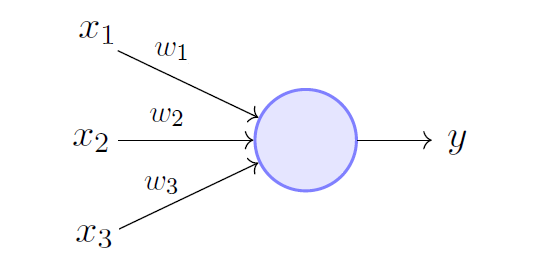
\includegraphics[scale=0.5]{perceptron2.png}
\caption{een enkelen perceptron}
\label{peceptron2}
\end{figure}
\linebreak
In afbeelding \ref{peceptron2} is een perceptron te zien die 3 variabelen als input neemt: $x_{1}, x_{2}$ en $x_{3}.$ Bij all deze waardes word een gewicht(weight) toegekend($w_{n}$). Deze waarde geeft aan hoe belangrijk de input is voor deze neuron. De output van de neuron is de som van alle resultaten bij elkaar. $\sum_{j}w_{j}x_{j}$ en deze waarde vergelijken met een gekozen randwaarde(threshold) om de output the berekenen. In een meer wiskundige term (w = weight, x = input en b = bias):

\begin{equation*}
\text{output perceptron}= \begin{cases}
0 &\text{if $\sum_{j}w_{j}x_{j}+ b \leq $ threshold }\\
1 &\text{if $\sum_{j}w_{j}x_{j}+ b>$ threshold }
\end{cases} 
\label{perceptron functie}
\end{equation*}
\newline
\noindent Je kan de output van een neuron beinvloeden door te spelen met de weights en thresholds. Door een input zijn weight te vergroten of de threshold te verlagen kan er hele andere resultaten uit het model komen\cite{NeuralNetwork1}. 
\newpage
\noindent Het is duidelijk dat de perceptron niet een compleet model is over hoe mensen hun beslissingen nemen. Maar het voorbeeld illustreert hoe een perceptron verschillende soorten bewijs kan afwegen om beslissingen te nemen. Daarom is het aannemelijk dat een complex netwerk van perceptrons vrij subtiele beslissingen zou moeten kunnen nemen\cite{NeuralNetwork1}.
\begin{figure}[h!]
\centering
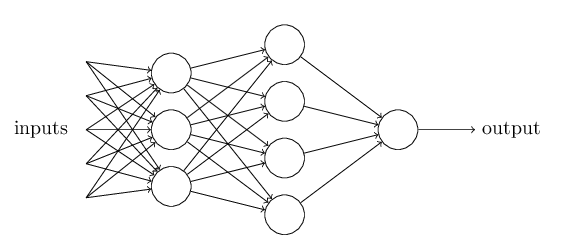
\includegraphics[scale=0.5]{perceptron3.png}
\caption{een neural network van meerderen perceptrons}
\label{perceptron3}
\end{figure}
\newline
In afbeelding \ref{perceptron3} is een netwerk te zien, waar de eerste laag van perceptrons in het netwerk, drie simpele beslissingen neemt door de functie in vergelijking \ref{perceptron fucntion} uit te voeren. Naast de eerste laag zit er nu ook een tweede die de outputs van de eerste laag als input neemt. Op deze manier kan een perceptron in de tweede laag een beslissing nemen op een complexer en abstracter niveau dan perceptrons in de eerste laag. Deze complexiteit en abstractheid word verhoogd per extra laag dat je toevoegd. Op deze manier kan een meerlaags netwerk van perceptrons, zeer geavanceerde beslissingen nemen\cite{NeuralNetwork1}\cite{learning}.\\ 
\newline
De volgende stap is om ons netwerk zelf lerend te maken. Om dit te doen moet je kleine aanpassingen kunnen maken aand de weights en de biases. Deze kleine aanpassingen moet daarna ook een klein effect hebben op de output van het neurale netwerk. Echter dat is niet wat er gebeurt met perceptronen want deze heeft maar 2 outputs, een 1 en een 0. Een kleine aanpassing zal daarom niks doen of de hele uitkomst van de perceptron omdraaien. Je kan niet probleem omzeilen door een ander types neurons te gebruiken ,zoals de Sigmoid en tanh neurons.\cite{learning}
\pagebreak
\subsubsection{Activatie functies}
De resultaten van een neuron worden berekend door een activatie functioes. Voor dit onderzoek worden eerst alleen de "Sigmoid" en "Tanh" activatie functies gebruikt, mochten deze niet goed werken worden andere activatie functies verder onderzocht\cite{learning}. \\\\
De sigmoid en tanh neurons lijken erg op perceptrons, alleen de manier hoe de ouput berekend wordt is compleet anders. Een sigmoid function neemt alle mogelijke nummers als een input en berekent het naar een getal tussen de 0 en 1.\\\\
\begin{equation}
    i_ \theta (x) =  \frac{\mathrm{1} }{\mathrm{1} + e^{-x} }  \label{sigmoid}
  \end{equation}
Een tanh functie neemt alle mogelijke nummers als input en brekend het naar en getal tussen de -1 en de 0.\\
\begin{equation}
    j_ \theta (x) =  \frac{\mathrm{2} }{\mathrm{1} + e^{-2x} } -1 \label{tanh}
  \end{equation}
  \linebreak
  \noindent De twee berekeningen lijken erg op elkaar, omdat tanh een geschaalde vorm is van de sigmoid functions.

\subsubsection{Zelf lerend netwerk}
Er is data nodig om een neuraal netwerk te trainen. Nadat deze data verzameld is kan er gebruik gemaakt worden van een methode die het neurale netwerk traint. Voorbeeld van zulke methodes zijn forward propagation, back propagation en resilent propagation. Het doel van deze algoritmes is om alle neuronen een weight en een bias te geven. Hoe dat in praktijk gaat hangt af van de dataset en welk algoritmn er gebruikt gaat worden, kort samengevat gaat het op deze manier\cite{learning}:
\begin{itemize}
\item De start waarden voor de weights en biases zijn vaak random.
\item De dataset wordt meegegeven aan het network en daar wordt data/resultaten uit gegenereerd.
\item Deze resultaten worden vergeleken met de verwachting en het foutpercentage/error wordt berekend.
\item Deze informatie wordt gebruikt om het het netwerk te tunen, zodat de error verminderd wordt.
\item De stappen worden herhaald tot het netwerk aan de eisen voldoet.
\end{itemize}

\subsubsection{Overfitting}
Neurale netwerken zijn erg kwetsbaar voor overfitting. Dit is als een neural netwerk alleen kan omgaan met de data uit een specifieke dataset en niet goed reageert op toekomstige waarnemingen\cite{algoritms}.\\ 
\newline
Overfiting onstaat door teveel factoren in het neurale netwerk op te nemen. Dit kan door heel veel specifieke data te geven aan het netwerk of door heel veel neuron te gebruiken die connecties gaan maken met die data. Als je deze dingen doet zal het netwerk altijd beter passend worden voor de gegevens die we al hebben, maar een betere pasvorm voor de beschikbare data betekent niet een betere prestatie\cite{algoritms}. \\
\newline
Dit klopt ook voor een netwerk met teweinig train data en/of neurons, als je er een te eenvoudig neural netwerk van maakt dan kan je het essentiele patroon in de data niet vastleggen. Een neural netwerk dat te gecompliceerd is word tegevoelig voor de specifiece data die we hadden vastgelegt. Als gevolg precies omdat het zo fijn is afgestemd op die specifieke train data gegeven word zal die voor oplossingen die met nieuwe informatie komen dan waar die me getrained is zwaar varieren en onbetrouwbare outputs geven\cite{algoritms}.\\
\newline
Dit is niet echt te verkomen, alleen door goed na tedenken over welke informatie je het netwerk zal laten geven, hoelang je het zal trainen en hoeveel neurons en layers het netwerk zal krijgen kan je zorgen dat je geen last krijgt van overfitting. De netwerken moet altijd getest worden of ze deze in de buurt komen van de resultaten die verwacht worden of dat ze inplaats daar van zijn getrained op test.\cite{algoritms}.

\pagebreak
\section{Resultaten}

Voor alle neuralnetwerken die er zijn getrained is er een standaard scoring methode gebruikt. Elke netwerk is getest op 3 verschillende race banen.
\begin{itemize}
\item Aalborg
\item Alpine 1
\item Alpine 2
\end{itemize}
Dit zijn alle 3 asphalt banen. die in goede mix van verschillende soorten bochten en rechten stukken hebben zodat we een netwerk kunnen testen op alle benodigde kwaliteiten. Er word genoteerd in hoeveel tijd het gekost heeft om 1 ronde te rijden, de maximum snelheid die het netwerk berijkt heeft, de schade die het heeft opgelopen en welke verzie van de stuk methode is gebruikt. All deze resultaten staan hier gedocumenteerd \ref{testresulaten}.
%Uitleg geven over de testresulaten, zie bijlage \ref{testresulaten}. 

Uit deze resultaten kwam het all heel snel naar voren dat de error waarde van een netwerk niet een goed refference punt was voor het meten van succes. Er zijn netwerken geweest met een zeer lage error waarde die zeer slecht scoorde op de punten die wij hebben vast gesteld voor een goed netwerk.
%Uitleg waarom we niks gedaan hebben met de errorwaarde tests.

%Uitleg waarom alleen Tanh  waardes
omdat de data die gebruikt word voor het sturen van de torcs auto tussen de -1 en 1 zit is het verstandig om gebruik te maken van de tanh functie. Omdat tanh alle reëel getal tussen de -1 en 1 kan hebben, dus waarden zoals -0.875 ... en 0.132. Dit zorgt ervoor dat de uitkomst van een neuron niet een simple een ja of nee is maar veel complexer getal dat van alles en nog wat kan betekenen. Nu als er een kleine verandering plaatsvind in de weights of biases van het neurale netwerk zullen deze kleine verandering ook te vinden worden in de output uiteindelijk zorgt dit ervoor dat het neurale netwerk zelf kan leren.\\\\
%Uitleg waarom we uiteindelijk alleen Encog hebben gebruikt (Doet Alex).


%Uiteindelijke keuze om 2 netwerken volledig handmatig te testen en vergelijken. 

%Gedeelte over de stuck methode, hoe die is gemaakt. Uitleg erover. (Doet Alex)
		
%Uiteindelijke keuze voor beste netwerk. (Alex )

%Wat hadden we beter kunnen doen, wat kan er verbeterd worden. 
\section{Conclusie}
%Samenvatting Resultaten en wat er nog verbeterd kan worden
\pagebreak
\section{Bijlages}
\subsection{Architectuurontwerp}
%Alex maakt een mooi plaatje
\subsection{Testplan}
Er zijn heel verschillende mogelijkheden voor het maken neurale netwerk. Het is daarom lastig om te zien wat een postive of negative invloed heeft. Daarom word elk getrainde neuraal netwerk  vergeleken om te kijken welke eigenschappen samen het beste werkt. Hierbij is het belangrijk dat de error waarde niet te hoog is maar ook niet telaag, het netwerk moet zo min mogelijk crashen, gemakkelijk herstelt na een crash en het snelste een parcours kan volgen. We zuullen de auto op de volgende criteria beoordelen:
\begin{itemize}
\item De tijd waarop de auto 1 lap rijd op de geslecteerde baan
\item Het aantal schaden dat de auto heeft aan het einde van 1 lap
\item De max snelheid die een auto behaald tijdens 1 lap
\end{itemize}
Alex to do! \\\
%Er zijn beste races toegevoegd, er kan gemakkelijk uitgerekend worden wat de error per parcours %is. Deze waardes kunnen dan vergeleken worden en hieruit kan de beste eruitgehaald worden. \\\\
%Om te kijken of het neurale netwerk crasht kan op de volgende manieren: 
Ook moet er gekenen worden naar hoevaak of hoe erg de auto zichzelf vastrijd in het het parkour. Dat kunnen we op de volgende manieren doen:
\begin{itemize}
\item Uitvoeren en kijken naar de damage in het scorebord aan het einde van de race. Hiervoor hoeft dus niet de race gevolgd te worden.
\item De race handmatig uitvoeren en opletten tijdens de race of de auto crasht. Hiervoor moet er naar de race gekeken worden door iemand.
\end{itemize}


\noindent Kijken of de auto gemakkelijk herstelt na een crash is eigenlijk alleen te doen door een race volledig te bekijken. Elke crashsituatie is uniek, dus het is niet zeker of het neurale netwerk zichzelf terug kan plaatsen op de weg. Er kan voor gekozen worden om de simulatie gelijk te laten crashen en kijken hoe dit oppakt of te races op een dirttrack. Hier zal die snel tegen een muur rijden, echter weet je niet of de unstuck methode hetzelfde werkt met verschillende omstandigheden. \\\\
Voor de laatste check kan gemakkelijk een script gerund worden, deze voert het neurale netwerk uit op een selectie van banen en noteert de tijd. Hiervoor is menselijke interactie niet nodig. Alleen bij het kiezen van het beste netwerk uiteindelijk. \\\\

\noindent Gedurende het testen wordt er gekeken welke testmethodes het beste werken en daar zullen we dan ook uiteindelijk mee gaan testen. In resultaten zal dit verder worden onderzocht. 

\pagebreak
\documentclass[pt,twoside,a4paper]{article}
\usepackage{graphicx} 
\usepackage[english]{babel}
\newcommand\tab[1][1cm]{\hspace*{#1}}
\usepackage{cite}
\usepackage[skip=2pt]{caption}
\graphicspath{ {resources/} } 
\begin{document}
\section{Stuck versions}
U = Unstuck
\begin{table}[h]
\centering
\begin{tabular}{llllll}
 \textbf{Version} & \textbf{U\_TIME\_LIMIT} & \textbf{MAX\_U\_ANGLE} & \textbf{MAX\_U\_SPEED} & \textbf{MIN\_U\_DIST}  & \textbf{MAX\_U\_DIST} \\ \hline
 1.0 & 2.0  & 30/(180*pi) & 5.0 & 0.9 & 0.2 \\
 2.0 & 2.0  & 30/(180*pi) & 5.0 & 0.9 & 0.3     \\
 &  &  &  &  &    \\
\end{tabular}
\end{table}
\newpage
\section{Race results}
\begin{table}[h]
\noindent
\begin{tabular}{llllll}
 \textbf{Map} & \textbf{Network} & \textbf{Time} & \textbf{Damage} & \textbf{Topspeed}  & \textbf{Stuck method} \\ \hline
 Aalborg & 20\_18\_16  & 1:48:94 & 441 & 172 & Version 1 \\
 Alpine 1 & 20\_18\_16 & 3:08:78  & 1461 & 204 & Version 2    \\
 Alpine 2 & 20\_18\_16 & 2:20:88  & 601 & 192 & Version 2    \\
 Aalborg & 20\_18\_16  & 1:48:94 & 441 & 172 & Version 2 \\ \hline
 Aalborg & 30\_24\_18  & DNF & - & - & Version 2 \\ \hline
 Aalborg & 200\_40  & 1:57:61 & 569 & 167 & Version 2 \\ 
 Alpine 1 & 200\_40 & 3:08:63 & 551 & 207 & Version 2    \\
 Alpine 2 & 200\_40 & DNF & - & - & Version 2   \\
 &  &  &  &  &    \\
\end{tabular}
\end{table}
\newpage
Commentaar: 200\_40 gaat niet goed om met de stuck methode.
\end{document}

\pagebreak
\subsection{Planning}
\label{uiteind-plan}
\begin{table}[h!]
\begin{tabular}{lrr}
 \textbf{Taak} & \textbf{Planning} & \textbf{Opgeverd} \\ \hline
 Requirements & 1 & 5 \\
 Testplan & 2 & 6 \\
 Persoonlijk verslag & 6 & 8 \\
 Onderzoek controller & 4 & 5 (\textit{np}) \\
 Eerste versie controller & 6 & 8 \\
 Testen en verbeteren & 7 & 7 (np) \\
 Tweede versie controller & 6 & 7 (\textit{np}) \\
 Groepsverslag controller & 7 & 7 (\textit{np}) \\
 Reflectieverslag & 8 & 8 (\textit{np})  \\
\end{tabular}
\caption{Uiteindelijke gerealiseerde planning in weken. \textit{np = nieuwe periode}}
\end{table}
\newpage
\subsection{Commitlog}
\label{commitlog}
%git log --color --graph --oneline > l.txt

\let\XXegroup\relax
\expandafter\def\csname XX[31\endcsname{%
  \bgroup\let\XXegroup\egroup\leavevmode\color{red}}
\expandafter\def\csname XX[1;31\endcsname{%
  \bgroup\let\XXegroup\egroup\leavevmode\bfseries\color{red}}
\expandafter\def\csname XX[32\endcsname{%
  \bgroup\let\XXegroup\egroup\leavevmode\color{green}}
\expandafter\def\csname XX[1;32\endcsname{%
  \bgroup\let\XXegroup\egroup\leavevmode\bfseries\color{green}}
\expandafter\def\csname XX[33\endcsname{%
  \bgroup\let\XXegroup\egroup\leavevmode\color{yellow}}
\expandafter\def\csname XX[1;33\endcsname{%
  \bgroup\let\XXegroup\egroup\leavevmode\bfseries\color{yellow}}
\expandafter\def\csname XX[34\endcsname{%
  \bgroup\let\XXegroup\egroup\leavevmode\color{cyan}}
\expandafter\def\csname XX[1;34\endcsname{%
  \bgroup\let\XXegroup\egroup\leavevmode\bfseries\color{cyan}}
\expandafter\def\csname XX[35\endcsname{%
  \bgroup\let\XXegroup\egroup\leavevmode\color{magenta}}
\expandafter\def\csname XX[1;35\endcsname{%
  \bgroup\let\XXegroup\egroup\leavevmode\bfseries\color{magenta}}
\expandafter\def\csname XX[36\endcsname{%
  \bgroup\let\XXegroup\egroup\leavevmode\color{blue}}
\expandafter\def\csname XX[1;36\endcsname{%
  \bgroup\let\XXegroup\egroup\leavevmode\bfseries\color{blue}}


\expandafter\def\csname XX[\endcsname{\XXegroup}
\catcode`\^^[=13
\def^^[#1m{%
\expandafter\ifx\csname XX#1\endcsname\relax
\typeout{XX#1}%
\else
\csname XX#1\endcsname
\fi}
\
\begin{verbatim}
* 7806e44 spelling check done and added my personal reports
* 58713e9 Add jar controller
* 180862b Alex verslagen toegevoegd
* 7cf3cfc conclusie verbetered
* ea0c81a Herscherven en bijlages toegevoegd
* f0e9fba testplan beetje herschreven en toevoeging gedaan aan vooronderzoek
* a0e2333 added some more comments too the code
* 6820fb2 kline verbeteringen gemaakr
* bf0e91d Resultaten aangepast en conclusie toegevoegd
* 7120db9 Voeg code bijlages toe en aanpassing resultaten
* c2dd3a6 resulaten verbeterd
* 0661252 Boekenclub toegevoegd
* 9d56e33 Refactor Vooronderzoek
* 8ccf041 overfitting verbetered en aan de resultaten gewerkt
*   e9865ea Merge
|\  
| * a1da85f worked on results
| * 4c15f46 gewerkt aan resulataten documenteren
| * c9e1bf6 test
* | 9a07ff7 Rewrite report
|/  
* 66f052a Revert "resulaten gewerkt"
* d353487 resulaten gewerkt
*   67c5544 x
|\  
| *   fab16c5 Fix somethign
| |\  
| | * 8b6637a wat dingen verbetered
| * | 62b9480 Spellingscontrole
| |/  
* | 0606c4f fixed math and citations
|/  
* 2a7c2c8 Resultaten toegevoegd
*   fc82466 Merge branch 'master' of https://github.com/ThomasAlakopsa/machine_learning
|\  
| * 7b970b2 project opzet verbeterd
* | 0c49b6d Add testresults
|/ 
\end{verbatim} 
\begin{verbatim}
* 60d5a2f Rewrite vooronderzoek
* 97ded02 Testen uitgevoerd
* 1791729 added citations
* 6712d55 vooronderzoek verzie 1
* 3112101 test plan verbeterd
* 8b9ffc4 Testplan verbeteren
* 73e7574 Projectopzet toegevoegd, daarnaast verder gegaan met onderzoek
* 88810a0 finished perspectron in vooronderzoek
* a560bed worked on perceptron explanation
* e1d4ef3 Add AdjustBreaks method, add validation sets
* 18492f9 Change break algoritmn
* 23d92b0 Add filtering scorebord
* e72aeff Add option to give file name
* 4a8bab8 finished documenting all the training results
* f98924e added all the new networks
* ad5b9cf Methode eerste versie
* 40a5a30 Add verify method
* aae00ab Break can't be less then 0
* cdacea0 Fix resume method
* 87a6cf2 Groepsverslag opzet opgezet
* f4f1786 Add 100_40
* 820c658 added fucntion that asks for name of the file or press enter to use default
* 54dd446 added 80_65_50_35 version 1, 2 and 3 and 44_33_33_22 version 1,2 and 3. all with documented results
* 2d21c56 addes the result of network 200_100_40 and 100_60_40
* 07ad208 Add new score
* 61f81b0 updated version of 200_100_40 and 100_60_40
*   54e3c40 Merge branch 'master' of https://github.com/ThomasAlakopsa/machine_learning
|\  
| * ae46afe Generate scoreboard pdf latex
| * 321361d Run new tests
* | c850536 added my networks
|/  
* 9247e8d Nieuwe trainde networks
* 7468141 add scoreboard and remove print
* 6fba598 add scoreboard and remove print
* e84e80c Change stuck method & add new training
* feb9b08 added the best network we have for now
* 2f0c7ed Add extra layer & stuck method
* f23e4e0 Add right train_data
* 567d067 Test
* 6117f60 Add neuralnetworks
* 5fb6117 Add runnable
* 8bb5459 Added Neural Network with Encog
* b6b5ec9 removed not needed files
* a7054b0 added .bbl .gz and .blg files in the git ignore
* 1bf3bd6 updated .gitignore and added folders for personal reports and a template for the final report
* 991ddb0 setting up work station / code is running
* b741a3f added the code from Elvira
* 0a4409a first commit
\end{verbatim}

\bibliographystyle{plain}
%\bibliography{IEEEabrv,references}
\bibliography{references}
\end{document}